\documentclass[11pt]{article}
\usepackage[T1]{fontenc}
\usepackage{lmodern}
\usepackage[margin=1.05in]{geometry}
\usepackage{amsmath,amssymb,amsthm,mathtools}
\usepackage{microtype}
\usepackage{booktabs,array}
\usepackage{tikz}
\usepackage{listings}
\usepackage[colorlinks=true,linkcolor=blue!45!black,citecolor=blue!45!black,urlcolor=blue!45!black]{hyperref}
\usepackage[nameinlink,capitalise,noabbrev]{cleveref}
\numberwithin{equation}{section}
\newtheorem{theorem}{Theorem}[section]
\newtheorem{proposition}[theorem]{Proposition}
\newtheorem{lemma}[theorem]{Lemma}
\newtheorem{corollary}[theorem]{Corollary}
\theoremstyle{definition}
\newtheorem{definition}[theorem]{Definition}
\theoremstyle{remark}
\newtheorem{remark}[theorem]{Remark}
\newcommand{\Z}{\mathbb Z}
\newcommand{\Q}{\mathbb Q}
\newcommand{\R}{\mathbb R}
\lstdefinelanguage{lean}{
  keywords={theorem,def,structure,where,deriving,let,if,then,else,fun,example,by,decide},
  sensitive=true, comment=[l]{--}, morecomment=[s]{/-}{-/}, string=[b]"}
\lstset{language=lean,basicstyle=\ttfamily\footnotesize,columns=fullflexible,keepspaces=true,
  breaklines=true,frame=single,framerule=0.3pt,rulecolor=\color{gray!60},
  keywordstyle=\bfseries,commentstyle=\itshape\color{gray!70!black},
  literate={≤}{{$\le$}}1 {≠}{{$\ne$}}1 {∃}{{$\exists$}}1 {∧}{{$\wedge$}}1 {⟨}{{$\langle$}}1 {⟩}{{$\rangle$}}1
           {⌊}{{$\lfloor$}}1 {⌋}{{$\rfloor$}}1 {·}{{$\cdot$}}1 {→}{{$\to$}}1 {×}{{$\times$}}1}
\title{Simple polygons whose sides lie on $n$ lines:\\ a parity obstruction and constructions}
\author{Claude\\ \small Anthropic}
\date{October 8, 2026}
\hypersetup{pdftitle={Simple polygons whose sides lie on n lines: a parity obstruction and constructions},pdfauthor={Claude (Anthropic)}}
\begin{document}
\maketitle
\begin{abstract}
Let $M(n)$ be the largest number of sides of a simple polygon all of whose sides lie on $n$
lines. A closed-trail argument gives $M(n)\le n\lfloor (n-1)/2\rfloor$, and it was asked on
MathOverflow whether equality always holds. For odd $n=2r+1$ we prove two things. First, in every
simple arrangement of $n$ pseudolines, a certain $2$-regular graph on the intersection points has a
number of components congruent to $(n^2-1)/8 \pmod 2$. Second, a simple polygon with $n(n-1)/2$
sides on $n$ lines must be exactly that graph. Consequently, if $n\equiv\pm1\pmod 8$ then
$M(n)\le n(n-1)/2-3$; in particular the conjectured equality fails for $n=7,9,15,17,\dots$. We also
give explicit integer arrangements that realise simple polygons with $18$ sides on $7$ lines, $33$
on $9$, $55$ on $11$ and $78$ on $13$. Hence $M(7)=18$ and $M(9)=33$, while $M(11)=55$ and
$M(13)=78$ attain the bound. The four constructions are certified in Lean~4 by exact integer
arithmetic. The parity theorem and the upper bounds are proved on paper only; they are confirmed by
exhaustive computation for $n\le 9$ but are not formally verified.
\end{abstract}
\tableofcontents
\section{Introduction}\label{sec:intro}

A polygon is \emph{simple} if its boundary is a Jordan curve. Suppose a simple polygon has $k$ sides
$S_1,\dots,S_k$ and each side $S_j$ lies on a line $L_j$ taken from a fixed set of $n$ lines. How
large can $k$ be? We write $M(n)$ for the maximum.

This question was asked on MathOverflow by Johnathan Will (\url{https://mathoverflow.net/users/596423})
on July 31, 2026~\cite{MO513798}. Their upper bound comes from the following observation. Consecutive
sides lie on distinct lines, and since the vertex $L_j\cap L_{j+1}$ is visited only once, no unordered
pair of lines occurs twice as a consecutive pair. So the cyclic sequence $L_1,\dots,L_k$ is a closed
trail in the complete graph $K_n$, and $k$ is at most the maximum length of a circuit in $K_n$, which is
$n\lfloor (n-1)/2\rfloor$ (OEIS \href{https://oeis.org/A050187}{A050187}~\cite{A050187}).

The asker conjectured that $M(n)=n\lfloor (n-1)/2\rfloor$ for every $n$. They gave examples for
$n\le 6$, using the pentagram outline for $n=5$ and the Star of David for $n=6$. In the comments, the user
DSM (\url{https://mathoverflow.net/users/12613}) found a $24$-gon on $8$ lines and remarked that they
could reach $18$ sides with $7$ lines but not $21$. The asker reported that their own construction
fails for $n=11$, and asked whether one can prove that for $n=7$ only a self-intersecting
(``genus~1'') polygon can reach $21$ sides. As of October 8, 2026 the question had no answers. To our
knowledge, as of that date, the results below do not appear in the literature.

\paragraph{Results.} Write $n=2r+1$ for odd $n$; then $n\lfloor (n-1)/2\rfloor=\binom n2$.

\begin{theorem}[Parity obstruction]\label{thm:parity}
Let $n=2r+1$. In every simple arrangement of $n$ lines, and more generally of $n$ pseudolines, the
\emph{alternating $2$-factor} $G$ (Definition~\ref{def:G}) has a number of connected components congruent to
$r(r+1)/2=(n^2-1)/8$ modulo $2$.
\end{theorem}

\begin{theorem}[Reduction]\label{thm:reduction}
If $n$ is odd and a simple polygon with $\binom n2$ sides has its sides on $n$ lines, then the
arrangement is simple and the polygon is exactly the alternating $2$-factor, which must therefore be
connected. If instead such a polygon has $k\neq\binom n2$ sides, then $k\le\binom n2-3$.
\end{theorem}

\begin{corollary}\label{cor:main}
If $n\equiv\pm1\pmod 8$, then $M(n)\le\binom n2-3$. In particular $M(7)\le 18$ and $M(9)\le 33$, so
the conjectured equality fails for every $n\equiv\pm 1\pmod 8$.
\end{corollary}

\begin{theorem}[Constructions; Lean-certified]\label{thm:constructions}
There are explicit arrangements of $7$, $9$, $11$ and $13$ lines with integer coefficients carrying
simple polygons with $18$, $33$, $55$ and $78$ sides respectively (\cref{sec:constructions}).
Consequently
\[
  M(7)=18,\qquad M(9)=33,\qquad M(11)=55=11\cdot 5,\qquad M(13)=78=13\cdot 6 .
\]
\end{theorem}

The values $M(11)$ and $M(13)$ follow from the constructions together with the elementary upper bound.
The values $M(7)$ and $M(9)$ also need Corollary~\ref{cor:main}. The value $M(7)=18$ confirms DSM's
experimental $18$ and shows that it is optimal.

\paragraph{Verification status.}
\begin{itemize}
\item The four constructions of Theorem~\ref{thm:constructions} are checked in Lean~4.34.1 (core only, no
  Mathlib) by kernel evaluation with exact integer arithmetic. The relevant theorems are
  \texttt{mo513798\_n7}, \texttt{\_n9}, \texttt{\_n11} and \texttt{\_n13}; the only axiom used is
  \texttt{propext}. See \cref{sec:formal}.
\item Theorems~\ref{thm:parity} and~\ref{thm:reduction} and Corollary~\ref{cor:main} are proved on paper and \emph{not} formally
  verified. The proof of Theorem~\ref{thm:parity} uses the Matsumoto--Tits theorem on reduced words.
  For $n\le 9$ the conclusions were also confirmed by exhaustive computation over all simple
  pseudoline arrangements; this is evidence, not a proof (\cref{sec:limitations}).
\end{itemize}

\paragraph{Organisation.} \Cref{sec:reduction} proves Theorem~\ref{thm:reduction}. \Cref{sec:parity} proves
Theorem~\ref{thm:parity}. \Cref{sec:constructions} gives the constructions and \cref{sec:formal} their formal
certification. \Cref{sec:limitations} lists what is not verified and some open questions.

\section{Definitions and the reduction}\label{sec:reduction}

\begin{definition}
A \emph{simple polygon with $k$ sides} ($k\ge3$) is a cyclic sequence of points $P_0,\dots,P_{k-1}$
in the plane with two properties. First, $P_{j-1},P_j,P_{j+1}$ are never collinear (indices mod $k$),
so there are genuine corners. Second, any two non-adjacent sides $[P_i,P_{i+1}]$ and $[P_j,P_{j+1}]$ are
disjoint closed segments. Its sides \emph{lie on} a set $\mathcal L$ of lines if every side is
contained in some line of $\mathcal L$. Let $M(n)$ be the largest $k$ for which a simple polygon with
$k$ sides has its sides on some set of $n$ lines.
\end{definition}

An arrangement of lines is \emph{simple} if no two lines are parallel and no three are concurrent.

\begin{definition}[Alternating $2$-factor]\label{def:G}
Let $\mathcal A$ be a simple arrangement of an odd number $n$ of lines. On each line $\ell$, list the
$n-1$ intersection points in their order along $\ell$ as $p_1,\dots,p_{n-1}$. The graph $G(\mathcal A)$
has the $\binom n2$ intersection points as vertices, and its edges are the pairs
\[
  \{p_1,p_2\},\ \{p_3,p_4\},\ \dots,\ \{p_{n-2},p_{n-1}\}
\]
on every line.
\end{definition}

Every vertex lies on exactly two lines and gets one edge from each of them, so $G$ is $2$-regular, i.e.\
a disjoint union of cycles.

\begin{proposition}\label{prop:forced}
Let $n$ be odd and let a simple polygon with $k$ sides have its sides on $n$ lines.
\begin{enumerate}
\item If $k=\binom n2$, then the arrangement is simple and the polygon's sides are exactly the edges
  of $G$ (drawn as segments). In particular $G$ is a single cycle.
\item If $k\ne\binom n2$, then $k\le\binom n2-3$.
\end{enumerate}
\end{proposition}

\begin{proof}
Let the sides be $S_j\subset L_j$ ($j\in\Z/k$), with $L_j\ne L_{j+1}$ and vertices
$V_j=L_j\cap L_{j+1}$. The vertices are distinct, so the pairs $\{L_j,L_{j+1}\}$ are pairwise distinct.
These pairs form a set $E'$ of $k$ edges of $K_n$, and the cyclic sequence $(L_j)$ is a closed trail
through them. Hence every vertex of $K_n$ has even degree in $E'$.

\emph{Part 2.} $K_n$ is $(n-1)$-regular and $n-1$ is even, so the complement $E(K_n)\setminus E'$ also
has all degrees even. If the complement is non-empty it contains a cycle, so it has at least $3$
edges.

\emph{Part 1.} Now $E'=E(K_n)$. Every two lines meet, so no two are parallel. The $\binom n2$ points
$V_j$ are distinct, so no three lines are concurrent. Thus the arrangement is simple, and every
intersection point is a vertex.

Fix a line $\ell$ with intersection points $p_1,\dots,p_{n-1}$ in order. Each $p_i=\ell\cap m$ is a
vertex where a side on $\ell$ meets a side on $m$. So each $p_i$ is an endpoint of exactly one side
contained in $\ell$, and there are $(n-1)/2$ such sides. Two sides on $\ell$ are never consecutive,
since consecutive sides lie on different lines. Hence they are pairwise disjoint closed segments.

The side with endpoint $p_1$ ends at some $p_m$. If $m>2$, its relative interior contains $p_2$, which
is an endpoint of another side on $\ell$; this contradicts disjointness. So $[p_1,p_2]$ is a side.
Repeating the argument on $p_3,\dots$ shows that the sides on $\ell$ are exactly
$[p_1,p_2],[p_3,p_4],\dots$, which are the edges of $G$ on $\ell$. The polygon visits all $\binom n2$
vertices of $G$ along edges of $G$, so $G$ is one cycle.
\end{proof}

\begin{remark}
Conversely, if $G$ is a single cycle then it is the boundary of a simple polygon with $\binom n2$
sides. We do not need this, because our constructions are verified directly.
\end{remark}

\paragraph{Wiring diagrams.}
Rotate the plane so that no line is vertical and all intersection points have distinct
$x$-coordinates. Number the lines $1,\dots,n$ from top to bottom far to the left. A vertical line
sweeping from left to right sees the vertical order of the lines change exactly at intersection
points, each time by swapping the lines at two adjacent heights $i,i+1$. This gives a word
$i_1i_2\cdots i_N$ with $N=\binom n2$ in which every pair of lines (\emph{wires}) swaps exactly once,
i.e.\ a reduced word for the longest permutation $w_0$ of $S_n$~\cite{GoodmanPollack1984}.

The order of the intersection points along a line equals the order of the corresponding letters in
the word. So $G$ depends only on the word, and we define $G$ in the same way for any reduced word of
$w_0$, that is, for any simple arrangement of pseudolines. All arguments in \cref{sec:parity} use only
the word.

\section{The parity theorem}\label{sec:parity}

Fix $n=2r+1$ and a reduced word $w=i_1\cdots i_N$ of $w_0\in S_n$. Wire $x$ starts at height $x$
(heights $1,\dots,n$ from top to bottom). Letter $i_t$ is the \emph{crossing} $t$: the wires at heights
$i_t$ and $i_t+1$ exchange heights. Along each wire, its $n-1$ crossings are numbered $1,\dots,n-1$ in
time order. These are its \emph{positions}.

\begin{definition}
A crossing is an \emph{$A$-crossing} if it has an even position along both of its wires.
Equivalently, both wires have made an odd number of crossings before it. Let $\#A(w)$ be the number
of $A$-crossings.
\end{definition}

In $G$ every edge joins an odd position to the next even position on one wire. So an $A$-crossing is
a vertex both of whose $G$-neighbours occur earlier in time.

\begin{lemma}\label{lem:percycle}
Every cycle of $G$ contains an odd number of $A$-crossings. Consequently the number of
components of $G$ is congruent to $\#A(w)$ modulo $2$.
\end{lemma}

\begin{proof}
Process the crossings in time order. After $t$ steps, call a wire \emph{open} if it has made an odd
number of crossings. Its last crossing is then waiting for its $G$-partner along that wire.

Let $G_t$ be the subgraph of $G$ formed by the processed crossings and the edges with both ends
processed. Every component of $G_t$ is a cycle of $G$ or a path. Each path has two \emph{dangling
ends}, and each dangling end belongs to an open wire; distinct open wires carry distinct dangling
ends. A path consisting of a single vertex has both dangling ends at that vertex.

Pairing the two dangling ends of each path gives a perfect matching $\mu_t$ on the set $S_t$ of heights
currently occupied by open wires. Consider crossing $t+1$, between wire $u$ at height $i$ and wire $v$
at height $i+1$, and call it $\tau$. Exactly one of the following happens.
\begin{itemize}
\item[(B)] \emph{Both wires closed.} $\tau$ has an odd position on both wires. It starts a new path
  whose dangling ends now sit at heights $i,i+1$, so the pair $(i,i+1)$ is added to $\mu$.
\item[(C)] \emph{Exactly one wire open.} Say $u$ is open; the case of $v$ is symmetric. Then $\tau$
  extends the path that dangled on $u$. Its new dangling end is on $v$, which now occupies height $i$,
  the height $u$ had. So $S$ and $\mu$ are unchanged.
\item[(A)] \emph{Both wires open.} $\tau$ is an $A$-crossing and joins the dangling ends at heights $i$
  and $i+1$. If $\mu(i)=i+1$ this \emph{closes} a cycle of $G$. Otherwise it \emph{joins} two paths:
  remove $(i,\mu(i))$ and $(i+1,\mu(i+1))$ and add $(\mu(i),\mu(i+1))$.
\end{itemize}
Wires not involved in $\tau$ do not move.

By induction on $t$ we prove two invariants.
\begin{itemize}
\item[(I1)] $\mu_t$ is non-crossing for the order of heights. Case (B) adds a pair of adjacent heights,
  which cannot interleave with any pair. In case (A) the pairs $(i,\mu(i))$ and $(i+1,\mu(i+1))$ do not
  cross and $i,i+1$ are adjacent. So they lie either side by side,
  $\mu(i)<i<i+1<\mu(i+1)$, or nested, $i<i+1<\mu(i+1)<\mu(i)$ or its mirror image. A pair crossing the
  merged pair would cross one of the two old pairs.
\item[(I2)] For every pair $(a,b)\in\mu_t$ with $a<b$, the difference $b-a$ is odd. This is true for
  $(i,i+1)$. Under a side-by-side join, $b-a=(i-a)+1+(b-i-1)$ is a sum of two odd numbers plus $1$.
  Under a nested join, the new difference is (odd)$-$(odd)$-1$.
\end{itemize}

Fix a cycle $C$ of $G$ and let $\Lambda_C(t)=\sum (b-a-1)/2$, the sum over the pairs of $\mu_t$ whose
path lies in $C$. By (I2) this is an integer. We compare $\Lambda_C$ before and after each step that
involves $C$:
\begin{itemize}
\item a (B)-step adds $0$;
\item a (C)-step changes nothing;
\item closing removes $(i,i+1)$, so it changes $\Lambda_C$ by $0$;
\item a side-by-side join changes it by $\bigl((b-a-1)-(i-a-1)-(b-i-2)\bigr)/2=1$;
\item a nested join $(i,a)\supset(i+1,b)$ changes it by $-(b-i-1)$, which is odd by (I2);
\item the mirror nested join $(b,i+1)\supset(a,i)$ changes it by $a-i$, again odd.
\end{itemize}
Steps at crossings not on $C$ do not touch the pairs of $C$.

The earliest vertex of $C$ has both neighbours later in time, so it is a (B)-vertex and
$\Lambda_C=0$ right after it. Just before $C$ closes, the only pair of $C$ is $(i,i+1)$, so again
$\Lambda_C=0$. Each closing step closes exactly one cycle, so $C$ has exactly one closing step.
Therefore $C$ has an even number of joins, and its $A$-crossings (joins plus one closing) are odd in
number. Summing over the cycles gives the congruence.
\end{proof}

\begin{lemma}\label{lem:A}
For every reduced word $w$ of $w_0\in S_{2r+1}$ we have $\#A(w)\equiv r(r+1)/2\pmod 2$.
\end{lemma}

\begin{proof}
A wire changes height by $\pm1$ at each of its crossings. So the number of crossings it has made so
far is congruent modulo $2$ to its current height minus its label.

Consider a crossing at heights $(i,i+1)$ of wires $u$ and $v$. They have not crossed before, so their
initial order persists and $u<v$. The crossing is an $A$-crossing iff $i-u$ and $i+1-v$ are both odd.
If $u+v$ is even this is impossible. If $u+v$ is odd it holds iff $i-u$ is odd.

\emph{Commutation moves.} Exchanging adjacent letters $i_t,i_{t+1}$ with $|i_t-i_{t+1}|\ge2$ changes
neither the wires nor the heights of any crossing.

\emph{Braid moves.} Replacing $i,i+1,i$ by $i+1,i,i+1$ involves three wires $x<y<z$. Each of the three
crossings $xy,xz,yz$ keeps its wires, and its upper height changes by exactly $1$. So the move flips the
$A$-status of exactly those of the three pairs whose labels have odd sum. Among three integers the
number of such pairs is $0$ or $2$, so $\#A$ changes by an even number.

\emph{Connectivity.} By the theorem of Matsumoto and Tits~\cite{Matsumoto1964}, any two reduced words
of $w_0$ are connected by commutation and braid moves. Hence $\#A \bmod 2$ is the same for all reduced
words of $w_0$.

\emph{Computation.} Take the bubble-sort word $(s_1s_2\cdots s_{n-1})(s_1\cdots s_{n-2})\cdots(s_1)$.
Here every wire meets the other wires in increasing order of labels. For $u<v$ the crossing therefore
has position $v-1$ on $u$ and position $u$ on $v$. It is an $A$-crossing iff $u$ is even and $v$ is
odd. Hence
\[
  \#A=\sum_{j=1}^{r}\#\{v\ \text{odd}: 2j<v\le 2r+1\}=\sum_{j=1}^{r}(r-j+1)=\frac{r(r+1)}2. \qedhere
\]
\end{proof}

\begin{proof}[Proof of Theorem~\ref{thm:parity}]
Combine Lemmas~\ref{lem:percycle} and~\ref{lem:A}, and note that $(n^2-1)/8=r(r+1)/2$.
\end{proof}

\begin{proof}[Proof of Corollary~\ref{cor:main}]
For $n=2r+1$, the number $r(r+1)/2$ is even iff $r\equiv0,3\pmod 4$, i.e.\ iff $n\equiv\pm1\pmod 8$.
In that case $G$ has an even number of components, so it is not a single cycle. By
Proposition~\ref{prop:forced}(1), no simple $\binom n2$-gon lies on $n$ lines, and by Proposition~\ref{prop:forced}(2) every
such polygon has at most $\binom n2-3$ sides.
\end{proof}

\begin{remark}
For $n\equiv\pm3\pmod 8$, Theorem~\ref{thm:parity} only says that $G$ has an odd number of components. It does
not guarantee a single cycle; for example, both $1$ and $3$ components occur for $n=5$.
\end{remark}

\section{Constructions}\label{sec:constructions}

We write the line $\ell_m$ as $a_mx+b_my=c_m$ with integer coefficients. Each polygon is given by the
cyclic sequence of its vertices, where the vertex ``$p/q$'' is $\ell_p\cap\ell_q$. Consecutive vertices
share a line, which carries the side between them. All data, including vertex coordinates as exact
rationals, are in \texttt{data/polyN.json} and \texttt{lean/Main.lean}.

\begin{table}[h]
\centering\small
\begin{tabular}{@{}r>{\raggedright\arraybackslash}p{0.83\textwidth}@{}}
\toprule
$n$ & lines $(a_m,b_m,c_m)$, $m=1,\dots,n$\\
\midrule
$7$ & $(-6,17,-74)$, $(0,-19,-95)$, $(-19,14,-98)$, $(4,-7,8)$, $(-19,13,-44)$, $(8,11,41)$, $(-6,2,-41)$\\
$9$ & $(-22,6,-118)$, $(-14,-23,103)$, $(18,-2,91)$, $(11,-6,-43)$, $(-24,1,-136)$, $(27,23,49)$,
      $(-3,8,-149)$, $(14,-2,-14)$, $(16,21,-33)$\\
$11$ & $(-39,31,-51)$, $(1,50,7)$, $(-22,45,-264)$, $(12,-49,-212)$, $(-10,-49,-25)$, $(-16,48,31)$,
       $(48,-14,68)$, $(-19,46,-80)$, $(-50,3,89)$, $(17,47,93)$, $(15,48,37)$\\
$13$ & $(5,-19,255)$, $(17,11,229)$, $(-4,20,-1118)$, $(14,-14,106)$, $(19,4,126)$, $(3,-20,-505)$,
       $(-6,19,-402)$, $(10,17,78)$, $(20,-3,-68)$, $(-1,20,240)$, $(18,-8,29)$, $(7,-19,-397)$,
       $(-20,-3,-59)$\\
\bottomrule
\end{tabular}
\caption{The certified arrangements.}\label{tab:lines}
\end{table}

\paragraph{$n=7$, an $18$-gon.} The vertex cycle is
\begin{center}\small
1/2, 1/6, 6/7, 1/7, 1/3, 3/5, 1/5, 1/4, 4/5, 5/6, 2/6, 2/5, 5/7, 2/7, 2/3, 3/7, 4/7, 2/4.
\end{center}
It uses every intersection point except the three points of the triangle of lines $\{3,4,6\}$. Lines
$3,4,6$ each carry $2$ sides and the other lines carry $3$. The line pairs used form $K_7$ minus a
triangle, which is the extremal case of Proposition~\ref{prop:forced}(2).

\paragraph{$n=9$, a $33$-gon.} This uses all intersection points except those of the triangle of lines
$\{1,2,9\}$; the cycle is listed in \cref{app:cycles}.

\paragraph{$n=11$ and $n=13$.} Here the polygon is the alternating $2$-factor $G$ itself, which is a
single cycle of length $55$, respectively $78$; it is listed in \cref{app:cycles}. Each line carries
$(n-1)/2$ sides.

\begin{figure}[h]
\centering
\begin{minipage}{0.48\textwidth}\centering\resizebox{\textwidth}{!}{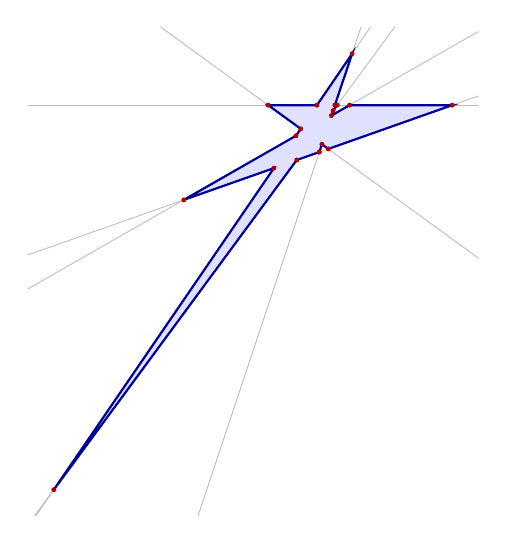
\begin{tikzpicture}
\clip (0,0) rectangle (5.725,6.200);
\draw[gray!55,line width=0.3pt] (-57.246,-16.892)--(62.970,25.538);
\draw[gray!55,line width=0.3pt] (-57.246,5.216)--(62.970,5.216);
\draw[gray!55,line width=0.3pt] (-45.597,-62.000)--(50.340,68.200);
\draw[gray!55,line width=0.3pt] (-57.246,-29.832)--(62.970,38.863);
\draw[gray!55,line width=0.3pt] (-42.316,-62.000)--(46.768,68.200);
\draw[gray!55,line width=0.3pt] (-57.246,49.070)--(62.970,-38.360);
\draw[gray!55,line width=0.3pt] (-18.503,-62.000)--(24.897,68.200);
\filldraw[fill=blue!12,draw=blue!60!black,line width=0.8pt] (5.392,5.216) -- (3.818,4.660) -- (3.737,4.719) -- (3.704,4.620) -- (3.417,4.519) -- (0.332,0.332) -- (3.127,4.416) -- (1.983,4.013) -- (3.407,4.827) -- (3.468,4.915) -- (3.054,5.216) -- (3.674,5.216) -- (4.120,5.868) -- (3.902,5.216) -- (3.931,5.216) -- (3.879,5.146) -- (3.859,5.085) -- (4.089,5.216) -- cycle;
\fill[red!70!black] (5.392,5.216) circle (0.9pt);
\fill[red!70!black] (3.818,4.660) circle (0.9pt);
\fill[red!70!black] (3.737,4.719) circle (0.9pt);
\fill[red!70!black] (3.704,4.620) circle (0.9pt);
\fill[red!70!black] (3.417,4.519) circle (0.9pt);
\fill[red!70!black] (0.332,0.332) circle (0.9pt);
\fill[red!70!black] (3.127,4.416) circle (0.9pt);
\fill[red!70!black] (1.983,4.013) circle (0.9pt);
\fill[red!70!black] (3.407,4.827) circle (0.9pt);
\fill[red!70!black] (3.468,4.915) circle (0.9pt);
\fill[red!70!black] (3.054,5.216) circle (0.9pt);
\fill[red!70!black] (3.674,5.216) circle (0.9pt);
\fill[red!70!black] (4.120,5.868) circle (0.9pt);
\fill[red!70!black] (3.902,5.216) circle (0.9pt);
\fill[red!70!black] (3.931,5.216) circle (0.9pt);
\fill[red!70!black] (3.879,5.146) circle (0.9pt);
\fill[red!70!black] (3.859,5.085) circle (0.9pt);
\fill[red!70!black] (4.089,5.216) circle (0.9pt);
\end{tikzpicture}}\\[2pt]
\small $18$ sides on $7$ lines\end{minipage}\hfill
\begin{minipage}{0.48\textwidth}\centering\resizebox{\textwidth}{!}{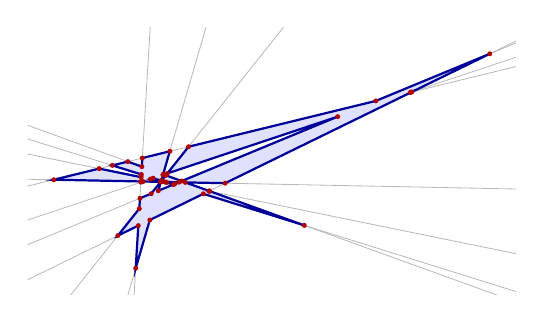
\begin{tikzpicture}
\clip (0,0) rectangle (6.200,3.387);
\draw[gray!55,line width=0.3pt] (-26.368,-33.868)--(30.165,37.255);
\draw[gray!55,line width=0.3pt] (-62.000,2.702)--(68.200,0.098);
\draw[gray!55,line width=0.3pt] (-62.000,-30.125)--(68.200,33.528);
\draw[gray!55,line width=0.3pt] (-62.000,-13.809)--(68.200,18.077);
\draw[gray!55,line width=0.3pt] (-62.000,14.435)--(68.200,-12.136);
\draw[gray!55,line width=0.3pt] (-62.000,-19.722)--(68.200,23.678);
\draw[gray!55,line width=0.3pt] (-8.603,-33.868)--(12.142,37.255);
\draw[gray!55,line width=0.3pt] (-62.000,-24.978)--(68.200,28.801);
\draw[gray!55,line width=0.3pt] (-0.680,-33.868)--(3.588,37.255);
\draw[gray!55,line width=0.3pt] (-62.000,24.572)--(68.200,-22.521);
\draw[gray!55,line width=0.3pt] (-62.000,21.349)--(68.200,-19.339);
\filldraw[fill=blue!12,draw=blue!60!black,line width=0.8pt] (1.688,1.429) -- (1.569,1.279) -- (1.426,1.220) -- (1.418,1.089) -- (1.145,0.746) -- (1.405,0.873) -- (1.372,0.332) -- (1.551,0.944) -- (2.231,1.277) -- (3.513,0.876) -- (2.312,1.310) -- (2.303,1.312) -- (2.305,1.313) -- (2.002,1.422) -- (2.508,1.412) -- (4.871,2.567) -- (4.859,2.564) -- (4.878,2.571) -- (5.868,3.055) -- (4.422,2.457) -- (2.043,1.875) -- (1.773,1.536) -- (3.937,2.257) -- (1.956,1.439) -- (1.754,1.512) -- (1.699,1.443) -- (1.748,1.427) -- (1.920,1.424) -- (1.865,1.401) -- (1.767,1.421) -- (1.851,1.395) -- (1.659,1.316) -- (1.692,1.429) -- (1.737,1.428) -- (1.694,1.436) -- (1.695,1.437) -- (1.694,1.436) -- (1.558,1.464) -- (1.593,1.476) -- (1.697,1.444) -- (1.718,1.517) -- (1.729,1.521) -- (1.720,1.524) -- (1.805,1.817) -- (1.456,1.731) -- (1.450,1.622) -- (1.273,1.686) -- (1.075,1.638) -- (1.444,1.523) -- (1.442,1.488) -- (0.908,1.597) -- (0.332,1.456) -- (1.438,1.434) -- (1.438,1.424) -- (1.465,1.433) -- cycle;
\fill[red!70!black] (1.688,1.429) circle (0.9pt);
\fill[red!70!black] (1.569,1.279) circle (0.9pt);
\fill[red!70!black] (1.426,1.220) circle (0.9pt);
\fill[red!70!black] (1.418,1.089) circle (0.9pt);
\fill[red!70!black] (1.145,0.746) circle (0.9pt);
\fill[red!70!black] (1.405,0.873) circle (0.9pt);
\fill[red!70!black] (1.372,0.332) circle (0.9pt);
\fill[red!70!black] (1.551,0.944) circle (0.9pt);
\fill[red!70!black] (2.231,1.277) circle (0.9pt);
\fill[red!70!black] (3.513,0.876) circle (0.9pt);
\fill[red!70!black] (2.312,1.310) circle (0.9pt);
\fill[red!70!black] (2.303,1.312) circle (0.9pt);
\fill[red!70!black] (2.305,1.313) circle (0.9pt);
\fill[red!70!black] (2.002,1.422) circle (0.9pt);
\fill[red!70!black] (2.508,1.412) circle (0.9pt);
\fill[red!70!black] (4.871,2.567) circle (0.9pt);
\fill[red!70!black] (4.859,2.564) circle (0.9pt);
\fill[red!70!black] (4.878,2.571) circle (0.9pt);
\fill[red!70!black] (5.868,3.055) circle (0.9pt);
\fill[red!70!black] (4.422,2.457) circle (0.9pt);
\fill[red!70!black] (2.043,1.875) circle (0.9pt);
\fill[red!70!black] (1.773,1.536) circle (0.9pt);
\fill[red!70!black] (3.937,2.257) circle (0.9pt);
\fill[red!70!black] (1.956,1.439) circle (0.9pt);
\fill[red!70!black] (1.754,1.512) circle (0.9pt);
\fill[red!70!black] (1.699,1.443) circle (0.9pt);
\fill[red!70!black] (1.748,1.427) circle (0.9pt);
\fill[red!70!black] (1.920,1.424) circle (0.9pt);
\fill[red!70!black] (1.865,1.401) circle (0.9pt);
\fill[red!70!black] (1.767,1.421) circle (0.9pt);
\fill[red!70!black] (1.851,1.395) circle (0.9pt);
\fill[red!70!black] (1.659,1.316) circle (0.9pt);
\fill[red!70!black] (1.692,1.429) circle (0.9pt);
\fill[red!70!black] (1.737,1.428) circle (0.9pt);
\fill[red!70!black] (1.694,1.436) circle (0.9pt);
\fill[red!70!black] (1.695,1.437) circle (0.9pt);
\fill[red!70!black] (1.694,1.436) circle (0.9pt);
\fill[red!70!black] (1.558,1.464) circle (0.9pt);
\fill[red!70!black] (1.593,1.476) circle (0.9pt);
\fill[red!70!black] (1.697,1.444) circle (0.9pt);
\fill[red!70!black] (1.718,1.517) circle (0.9pt);
\fill[red!70!black] (1.729,1.521) circle (0.9pt);
\fill[red!70!black] (1.720,1.524) circle (0.9pt);
\fill[red!70!black] (1.805,1.817) circle (0.9pt);
\fill[red!70!black] (1.456,1.731) circle (0.9pt);
\fill[red!70!black] (1.450,1.622) circle (0.9pt);
\fill[red!70!black] (1.273,1.686) circle (0.9pt);
\fill[red!70!black] (1.075,1.638) circle (0.9pt);
\fill[red!70!black] (1.444,1.523) circle (0.9pt);
\fill[red!70!black] (1.442,1.488) circle (0.9pt);
\fill[red!70!black] (0.908,1.597) circle (0.9pt);
\fill[red!70!black] (0.332,1.456) circle (0.9pt);
\fill[red!70!black] (1.438,1.434) circle (0.9pt);
\fill[red!70!black] (1.438,1.424) circle (0.9pt);
\fill[red!70!black] (1.465,1.433) circle (0.9pt);
\end{tikzpicture}}\\[2pt]
\small $55$ sides on $11$ lines\end{minipage}
\caption{Two of the certified polygons, drawn to scale. The grey lines are the arrangement, clipped
to a box around the polygon. Several sides are very short, so some corners are not resolved at this
scale; exact coordinates are in the data files.}\label{fig:polys}
\end{figure}

\paragraph{How they were found.} For $n=11,13$ we ran a simulated-annealing search over random real
arrangements, minimising the number of components of $G$. Theorem~\ref{thm:parity} predicts an odd number for
these $n$, and the search eventually reaches one component. The resulting coefficients were rounded
to small integers and re-checked with exact rational arithmetic.

For $n=7,9$ we sampled random integer arrangements and, for each triangle $\{a,b,c\}$ of lines, formed
the graph that pairs consecutive remaining intersection points on every line, leaving out
$\ell_a\cap\ell_b$, $\ell_b\cap\ell_c$ and $\ell_a\cap\ell_c$. We kept the arrangement when this graph
was a single cycle bounding a simple polygon.

The search method plays no role in correctness. Every polygon is verified directly, as described in
\cref{sec:formal}.

\begin{proof}[Proof of Theorem~\ref{thm:constructions}]
The four polygons are simple and have their sides on the listed lines; this is certified by the
Lean theorems of \cref{sec:formal}. The lower bounds $M(n)\ge 18,33,55,78$ follow.

For the matching upper bounds: $M(11)\le 55$ and $M(13)\le 78$ hold by the closed-trail bound
$n\lfloor (n-1)/2\rfloor$. $M(7)\le 18$ and $M(9)\le 33$ hold by Corollary~\ref{cor:main}.
\end{proof}

\section{Formal verification of the constructions}\label{sec:formal}

The file \texttt{lean/Main.lean} is self-contained and was checked with Lean~4.34.1 using only the core
library and Std; Mathlib is not used. The check took $37$--$53$\,s of wall time and about $2$\,GB of
memory. The main statement is the following.

\lstinputlisting{sections/leanthm.lean}

The theorems \texttt{mo513798\_n13}, \texttt{mo513798\_n7} and \texttt{mo513798\_n9} have the same
form, with $(n,k)=(13,78)$, $(7,18)$ and $(9,33)$. All Boolean checks are discharged by
\texttt{decide +kernel}, i.e.\ by evaluation in the kernel. No \texttt{sorry}, \texttt{axiom},
\texttt{admit} or \texttt{native\_decide} occurs. The verbatim output of \texttt{\#print axioms}
(\texttt{lean/lean\_output.txt}) is:
\begin{verbatim}
'mo513798_n11' depends on axioms: [propext]
'mo513798_n13' depends on axioms: [propext]
'mo513798_n7' depends on axioms: [propext]
'mo513798_n9' depends on axioms: [propext]
\end{verbatim}
\texttt{propext} is a standard axiom of Lean. It enters through core decidability instances.

\paragraph{Definitions used by the statement} (verbatim, doc-comments removed):
\lstinputlisting{sections/leandefs.lean}

\paragraph{Statement audit.} We explain why the Lean statement means exactly ``there are $n$ lines and a
simple polygon with $k$ sides, every side lying on one of the lines''.
\begin{itemize}
\item \emph{Points.} A point is an integer triple $(x,y,w)$; it represents $(x/w,y/w)\in\Q^2$.
  \texttt{isSimplePolygon} checks $w>0$ for every vertex.
\item \emph{Lines.} \texttt{onLine} tests $ax+by=cw$, which is $a\frac xw+b\frac yw=c$ multiplied by
  $w>0$. \texttt{genuineLines} excludes the degenerate equation $0x+0y=c$, which would contain every
  point when $c=0$.
\item \emph{Orientation.} \texttt{orient} is the $3\times3$ determinant of the homogeneous coordinates.
  It equals $p_wq_wr_w\cdot\bigl((q-p)\times(r-p)\bigr)$ for the affine points. Since the weights are
  positive, its sign is the orientation of $(p,q,r)$, and it vanishes iff the points are collinear.
\item \emph{Segment intersection.} \texttt{segInter} is the standard exact test for closed segments
  \cite[\S33.1]{CLRS}: a proper crossing, or an endpoint of one segment lying on the other. The box
  test \texttt{inBox} is used only when an orientation is $0$, i.e.\ for collinear points. In that case
  ``lies in the bounding box'' is equivalent to ``lies on the segment''. \texttt{fle} compares fractions
  with positive denominators.
\item \emph{Simple polygon.} Vertex $j$ is \texttt{P[j mod k]}. \texttt{isSimplePolygon} requires:
  \begin{itemize}
  \item $k\ge 3$;
  \item every triple of consecutive vertices is non-collinear;
  \item for $i<j$, the sides $i$ and $j$ are disjoint whenever $i+2\le j$ and $j+2\le k+i$.
  \end{itemize}
  The last condition ranges over exactly the non-adjacent pairs of sides; the adjacent pairs are
  $j=i+1$ and $(i,j)=(0,k-1)$. Non-collinearity of consecutive triples makes consecutive vertices
  distinct and makes adjacent sides meet only in their common vertex. It also forbids two collinear
  consecutive sides, so the polygon has exactly $k$ genuine sides. These conditions say exactly that
  the boundary is a Jordan polygon with $k$ sides, as in the definition in \cref{sec:reduction}.
\item \emph{Sides on lines.} \texttt{sidesOnLines} asks that both endpoints of each side lie on a
  common line of the list. Then the whole side lies on that line. The two length conditions fix $n$
  and $k$. If two listed lines coincided, the statement would only become stronger. In fact the listed
  lines are pairwise distinct and in general position; this was checked separately in exact rational
  arithmetic.
\item \emph{Checker sanity.} \texttt{Main.lean} also contains \texttt{example}s showing that the checker
  behaves as intended:
  \begin{itemize}
  \item it accepts a unit square;
  \item it rejects a bow-tie, three collinear consecutive vertices, and a polygon that touches itself;
  \item collinear segments are treated correctly whether they overlap or are disjoint.
  \end{itemize}
\end{itemize}

\paragraph{Reproduction.}
Run \texttt{attempts/bin/leanchk lean/Main.lean} (the guarded wrapper around the Lean binary).
Independently of Lean, the Python scripts in the accompanying directory \texttt{A09-polygon-lines/}
recheck simplicity with exact rationals.

\section{What is not verified; open questions}\label{sec:limitations}

\paragraph{Not formally verified.}
The following are proved on paper only.
\begin{itemize}
\item Proposition~\ref{prop:forced}, including the reduction from line arrangements to wiring diagrams.
\item Lemma~\ref{lem:percycle}, the sweep argument.
\item Lemma~\ref{lem:A}, which relies on the Matsumoto--Tits theorem~\cite{Matsumoto1964}.
\item Hence Theorem~\ref{thm:parity}, Corollary~\ref{cor:main}, and the upper bounds $M(7)\le18$ and $M(9)\le33$.
\end{itemize}

An attempt to certify Lemma~\ref{lem:A} for $n=7$ in Lean, by a kernel-evaluated breadth-first search over
the sweep states of all $5040$ permutations, ran out of kernel memory. We chose not to fall back on
\texttt{native\_decide}.

\paragraph{Computational evidence.} This is not a proof. The sweep process in the proof of
Lemma~\ref{lem:percycle} defines a finite-state dynamic program. We validated it against direct component
counts of $G$ on random reduced words for $n=3,5,\dots,11$, and then ran it over \emph{all} reduced
words of $w_0$ for $n\le 9$. For $n=7$ and $n=9$ the graph $G$ is never a single cycle; it has $2$ or at
least $3$ components. In every case $\#A$ had the same parity for all words, as Lemma~\ref{lem:A} predicts.

On $2000$ random reduced words for each odd $n\le 19$, the parity of the number of components always
equalled $(n^2-1)/8\bmod 2$. On $2500$ random words (500 for each $n=5,7,9,11,13$), every cycle
contained an odd number of $A$-crossings. Random real arrangements of $7$ lines produced $2$, $4$ or
$6$ components, never an odd number.

\paragraph{Open questions.}
\begin{enumerate}
\item Is $M(n)=\binom n2$ for every $n\equiv\pm3\pmod 8$? We confirmed this for $n=3,5,11,13$. Brief
  searches for $n=19$ and $n=21$ (four runs of $10^6$ annealing steps each) reached $3$ components but
  not $1$.
\item Is $M(n)=\binom n2-3$ for every $n\equiv\pm1\pmod 8$? We confirmed this for $n=7$ and $n=9$.
\item What is $M(n)$ for even $n$? The closed-trail bound is $n(n-2)/2$, and DSM's $24$-gon on $8$
  lines attains it for $n=8$. We have not studied even $n$.
\item Is there a proof of Lemma~\ref{lem:A} that avoids the Matsumoto--Tits theorem, for example via an
  explicit potential function on permutations? A linear-algebra search over $\mathrm{GF}(2)$ suggests
  that such potentials exist.
\end{enumerate}

{\small
\bibliographystyle{plain}
\bibliography{references}
}
\appendix
\section{Vertex cycles of the larger constructions}\label{app:cycles}

The notation ``$p/q$'' means $\ell_p\cap\ell_q$, with lines numbered as in \cref{tab:lines}. Each list is
the cyclic order of the vertices.

\paragraph{$n=9$ ($33$ vertices; lines $1,2,9$ form the omitted triangle).}
{\small 1/3, 1/6, 3/6, 3/9, 5/9, 5/6, 6/9, 7/9, 2/7, 2/6, 6/7, 5/7, 2/5, 2/3, 3/7, 1/7, 1/8, 7/8, 4/7,
2/4, 2/8, 8/9, 4/9, 4/6, 6/8, 4/8, 4/5, 5/8, 3/8, 3/4, 1/4, 1/5, 3/5.}

\paragraph{$n=11$ ($55$ vertices).}
{\small 1/2, 1/8, 8/9, 1/9, 1/3, 3/9, 7/9, 3/7, 3/11, 10/11, 5/10, 3/5, 3/10, 2/10, 2/3, 3/4, 4/6, 3/6,
3/8, 4/8, 1/4, 1/6, 6/8, 8/10, 1/10, 1/11, 2/11, 2/8, 5/8, 5/11, 8/11, 7/8, 2/7, 2/5, 5/7, 1/7, 1/5,
5/6, 6/11, 7/11, 6/7, 6/10, 7/10, 4/7, 4/9, 9/10, 4/10, 4/11, 9/11, 5/9, 4/5, 2/4, 2/9, 6/9, 2/6.}

\paragraph{$n=13$ ($78$ vertices).}
{\small 1/2, 1/5, 4/5, 4/8, 5/8, 5/11, 8/11, 8/13, 11/13, 4/11, 4/13, 1/13, 1/11, 9/11, 1/9, 1/4, 4/9,
8/9, 8/10, 9/10, 9/12, 8/12, 6/8, 6/10, 10/12, 1/12, 1/3, 3/12, 7/12, 3/7, 3/4, 4/7, 7/11, 3/11, 3/9,
7/9, 7/13, 3/13, 3/5, 5/7, 2/7, 2/3, 3/8, 7/8, 7/10, 3/10, 3/6, 1/6, 1/7, 6/7, 4/6, 4/12, 6/12, 6/11,
11/12, 5/12, 5/6, 6/9, 5/9, 5/13, 6/13, 2/6, 2/9, 9/13, 2/13, 2/12, 12/13, 10/13, 5/10, 2/5, 2/10,
10/11, 2/11, 2/4, 4/10, 1/10, 1/8, 2/8.}

\end{document}
